\documentclass{sprawozdanie-agh}

\usepackage[utf8]{inputenc}
\usepackage{listings}
\usepackage{pdfpages}
\usepackage{float}
\usepackage{anyfontsize}
\usepackage{graphicx}
\usepackage{multicol}

\setlength\columnsep{1cm}

\makeatletter

\begin{document}

	\przedmiot{Modelowanie i symulacja systemów}
	\tytul{„Traffic Sim”}
	\podtytul{Symulacja ruchu samochodów w mieście}
	\kierunek{Informatyka, III rok, 2018/2019}
	\autor{Konrad Gębczyński, Agnieszka Zadworny, Maciej Bielech}
	\data{Kraków, 13 grudnia 2018}

	\stronatytulowa{}

	% Spis treści

	\tableofcontents




	% Tekst właściwy
	\newpage
	\setlength{\parindent}{0pt} % usunięcie wcięcia we wszystkich paragrafach

	\section{Wstęp}

	Rozwój sektora transportu spowodował znaczny wzrost ilości pojazdów poruszających się po ulicach miast. Wiąże się to z wzmożonym ruchem, utrudniającym sprawne przemieszczanie się. Rozbudowa sieci dróg jest jednym z rozwiązań tego problemu, lecz istnieją też inne sposoby na usprawnienie ruchu ulicznego, takie jak inteligentne sygnalizacje świetlne, skrzyżowania bezkolizyjne, systemy badające ruch w czasie rzeczywistym i sterujące nim w zależności od potrzeb.

	Symulacje ruchu drogowego pozwalają sprawdzić jaki wpływ na układ drogowy będzie miał np. ruch generowany z projektowanego biurowca albo nowo budowanej drogi. Poza możliwościami jakie daje mikrosymulaja ruchu w 2D przeprowadzane symulacje mogą mieć  jeszcze bardziej przystępną formę. Wyniki symulacji mogą być przedstawione w postaci np. długości kolejek czy starty czasu, które są czytelne przede wszystkim dla inżynierów ruchu. Dodatkowo symulacje ruchu drogowego umożliwiają przedstawienie docelowej sytuacji w trzech wymiarach. Pozwala to na zobrazowanie inwestorowi czy zarządcy ruchu jak wygląda rozkład ruchu na okolicznych ulicach przy projektowanym obiekcie handlowym czy powstającym właśnie biurowcu, a obrazowane w ten sposób wyniki są dostępne dla osób, które na co dzień nie mają do czynienia z inżynierią ruchu.

	Symulacje ruchu pozwalają zobrazować przyszłą sytuację ruchową i przedstawić ja w przystępnej formie. Co więcej stanowią element, który na prezentacjach ma za zadanie przyciągać wzrok i uwagę widza, ponieważ pojazdy na symulacji poruszają się jak prawdziwe pojazdy, a decyzje poszczególnych pojazdów odzwierciedlają zachowania kierowców na drodze.

	Symulacje umożliwiają symulowanie jednocześnie ruchu samochodów, pieszych, rowerzystów, a także tramwajów. Dzięki temu możliwe jest umieszczenie, w jednej symulacji, wszystkich uczestników ruchu oraz przedstawienie wzajemnej interakcji między nimi.

	Tematem niniejszej pracy jest zamodelowanie i zasymulowanie jednego ze sposobów ograniczania zatorów, mianowicie skrzyżowania bezkolizyjnego. W pracy poruszymy takie kwestie jak: automaty komórkowe, model Nagela-Schreckenberga, czy listy kolejkujące.

	\section{Automaty komórkowe}

	Automat komórkowy wykorzystywany jest w różnorakich symulacjach. Automaty komórkowe definiowane są najczęsciej na dwa sposoby:

	\begin{itemize}
		\item Definicja Ferbera
		\begin{quote}
			Automaty komórkowe są dyskretnym, dynamicznym systemem, którego zachowanie jest całkowicie określone w warunkach lokalnych relacji
		\end{quote}
		\item Definicja Weimera
		\begin{quote}
			Automat komórkowy to czwórka $(L,N,S,f)$, gdzie
			\begin{itemize}
				\item L - przestrzeń podzielona na siatkę komórek,
				\item S - zbiór skończonych stanów,
				\item N - zbiór sąsiadów danej komórki,
				\item f - funkcja zmiany konfiguracji w poszczególnych komórkach.
			\end{itemize}
		\end{quote}
	\end{itemize}

	W ogólności automat komórkowy to matematyczny model dyskretny, dynamicznych procesów zachodzących w czasie. Rozpatrywana przestrzeń w naszej aplikacji będzie listą pozycji na których może znajdować się pojazd na drodze. Stan komórki będzie zmieniał się w dyskretnych chwilach czasu, podczas gdy samochody będą się poruszać. Ruch pojazdu zależał będzie od prędkości maksymalnej, jaką można poruszać się na drodze, od odległości od najbliższego sąsiada poruszającego się tym samym pasem ruchu oraz od poprzedniego stanu w jakim znajdował się rozpatrywany samochód. Warunkiem brzegowym naszej przestrzeni będzie dojechanie do sygnalizacji świetlnej lub końca drogi, w takiej sytuacji kierowca oczekuje na zmianę sygnalizacji, lub wybiera ulicę którą chce podrózować dalej.

	Automaty komórkowe pozwalają łączyć wielkie liczby komponentów, a także poziomów organizacyjnych w model umożliwiający bardzo szybką symulację zachowań systemu złożonego. Modele ruchu, które są oparte na automatach komórkowych to systemy dynamiczne, gdzie droga, czas oraz stany systemu stanowią wielkości dyskretne. Ewolucja modelu określana jest za pomocą reguł uaktualniania, które działają lokalnie (w sąsiedztwie danej komórki). W metodzie modelowania ruchu drogowego, bazującej na automatach komórkowych, droga została podzielona na komórki o stałej długości, natomiast pojazdy reprezentowane są przez punkty, które posiadają niezbędny zestaw parametrów. Co pewien stały krok czasowy każdy pojazd przemieszcza się zgodnie z regułami rządzącymi jego zachowaniem. Automaty komórkowe ze względu na swoją prostotę stanowią popularne narzędzie mikroskopowego modelowania ruchu drogowego. Modele wykorzystujące automaty komórkowe posiadają dużą wydajność obliczeniową. Ponad to, oferują możliwość odwzorowana i symulowania rzeczywistych zjawisk ruchu drogowego z zadowalającą dokładnością. Pozwalają również na realistyczne odwzorowanie środowiska ruchu miejskiego. Co więcej, umożliwiają one prognozę parametrów, które stanowią podstawę optymalizacji adaptacyjnego sterowania ruchem.


	\section{Symulacyjne modele ruchu}

	Bezpieczeństwo ruchu drogowego determinowane jest cechami infrastruktury drogowej oraz warunkami ruchowymi występującymi na sieci drogowej. Źle zaprojektowany układ sieci drogowej daje użytkownikom poważne trudności i przyczynia się do obniżenia bezpieczeństwa ruchu drogowego. Stosowane obecnie metody analiz ruchu drogowego, bazujące na matematycznych modelach makro i mikrosymulacji ruchu drogowego, umożliwiają racjonalne kształtowanie przebudowy i rozwoju układu drogowego, dostarczają niezbędne dane potrzebne do oceny poziomu warunków i bezpieczeństwa ruchu.

	Zapis zachodzcych w ruchu drogowym procesów pomiędzy pojazdami można ogólnie przedstawić w formie implikacji: $akcja \rightarrrow reakcja$ w określonym czasie obserwacji t:

	\begin{equation}
		Reakcja(t)=czulosc*bodziec(t-T)
	\end{equation}
	gdzie: T - czas reakcji na bodziec \\*

	W dzisiejszych czasach rozbudowujące się sieci drogowe, które są uwarunkowane rosnącym zapotrzebowaniem na przestrzeń transportową, stawiają przed inżynierami ruchu ogromne wyzwania. Jednym z nich jest konieczność osiągnięcia jak najwyższego poziomu bezpieczeństwa ruchu drogowego. Sprostanie tym zadaniom wymaga stosowania w projektowaniu i zarządzaniu ruchem najnowocześniejszych narzędzi, którymi są symulacyjne modele ruchu drogowego.
	W pracy skupiono się na mikrosymulacji wybranych skrzyżowań z sygnalizacją świetlną znajdujących się na terenie Krakowa. Teraz w kilku zdaniach przedstawione zastaną dwa modele symulacyjne ruchu drogowego – makro i mikrosymulacja.

	Pierwsze modele symulacyjne ruchu drogowego zostały zastosowane w połowie XX w. i były one modelami bardzo prostymi, posiadającymi szereg założeń upraszczających ich działanie. Symulacje te głównie dotyczyły przepływu ruchu na odcinkach międzywęzłowych sieci. Rozwój informatyki, a zwłaszcza numerycznych technik obliczeniowych sprzężonych z komputerami o coraz większej mocy obliczeniowej, przyczynił się do rozwoju nowocześniejszych procedur obliczeniowych stosowanych w inżynierii ruchu drogowego. W związku z tym rozwojem, w procedurach tych zaczęto uwzględniać coraz to większą grupę czynników wpływających na transport, a co za tym idzie na ruch drogowy. Procedury te mają za zadanie odwzorować skomplikowane zjawisko, jakim jest realizacja podróży w sposób możliwie dokładny i obrazujący stan istniejący. W myśl zasady „od ogółu do szczegółu” techniki symulacyjne wykształciły dwa poziomy analiz:

	\begin{itemize}
		\item makrosymulacje - w ujęciu sieciowym;
		\item mikrosymulacje – w ujęciu lokalnym.
	\end{itemize}


	\textbf{Makrosymulacje} dotyczą głównie dużego obszaru sieci transportowej tj. kraju (krajowy model ruchu drogowego), województwa bądź grupy województw (regionalny model ruchu drogowego), albo całego miasta (miejski model ruchu drogowego). W modelach takich proces transportowy odzwierciedla się za pomocą czterech kroków (model czterostopniowy):

	\begin{itemize}
		\item  Generowanie ruchu – tworzenie podróży wynikających z potrzeb człowieka (podróże indywidualne, transportem publicznym) oraz wynikające z potrzeb gospodarczych (np.: ruch pojazdów dostawczych). Opisane jest w ramach poszczególnych motywacji podróży: dom – praca, praca – dom itd.;
		\item Rozkład przestrzenny ruchu - wybór celu podróży związanego z zagospodarowaniem przestrzennym analizowanego obszaru;
		\item Wybór środka transportu do realizacji podróży (podział modalny) – opis kryteriów wyboru poszczególnych środków transportowych do realizacji podróży;
		\item Rozkład podróży/potrzeb transportowych na sieć transportową – określenie tras podróży w ramach poszczególnych systemów transportowych, a w konsekwencji natężeń ruchu i potoków pasażerskich w środkach transportowych.
	\end{itemize}

	Pierwsze trzy kroki modelowania pozwalają na określenie potrzeb transportowych mieszkańców w ramach danego systemu transportowego. Dzięki temu możliwa jest odpowiedź na pytanie: „Ile osób w danym przedziale czasu zamierza podróżować i jakim środkiem transportowym?”. Czwarty krok to określenie tras realizacji podróży. Pomiędzy poszczególnymi krokami obliczeniowymi istnieje ścisła zależność, ponieważ forma realizacji podróży zależy od możliwości jej realizacji, a także stopnia obciążenia ruchem sieci.

	\begin{figure}[H]
		\centering
		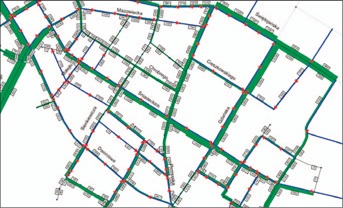
\includegraphics[width=0.8\textwidth]{Makrosymulacja.jpg}
		\caption{\textit{Wynik makrosymulacji ruchu dla wybranego obszaru sieci drogowej centrum Bydgoszczy}}
		[źródło: http://www.klir.pl/biuletyny/biuletyn70.pdf]
		\label{fig:Makrosymulacja}
	\end{figure}

	Efektem stosowania makrosymulacji jest uzyskanie danych o natężeniach ruchu dla całej sieci transportowej analizowanego układu. Pozwala to na określenie zmian natężeń ruchu drogowego i potoków pasażerskich np. dla budowy nowego odcinka drogi, wprowadzenia nowego systemu opłat za przejazd. \\*


	\textbf{Mikrosymulacje} dotyczą wybranego, najczęściej ograniczonego do kilku skrzyżowań i odcinków międzywęzłowych, obszaru sieci transportowej. Mikrosymulacje mogą odnosić się do różnych obszarów transportu, m.in. ruchu drogowego dla którego prowadzone są symulacje ruchu pojazdów na poszczególnych pasach ruchu. Mikrosymulacja to uzupełnienie markosymulacji przez uszczegółowienie zjawiska ruchu drogowego. Symulacje te obrazują sposób przemieszczania się pojazdów wskazując możliwe miejsca potencjalnych utrudnień w ruchu drogowym np.: zatory, czy długości kolejek na poszczególnych pasach ruchu drogowego.
	Techniki mikrosymulacji to świetne narzędzie prezentacji sytuacji ruchowej, a także pokazania możliwych konsekwencji zmian w organizacji ruchu drogowego polegających min. na wprowadzeniu dodatkowego pasa ruchu dla relacji prawoskrętu, czy też zmiany długości cyklu sygnalizacji świetlnej. Efektem mikrosymulacji zazwyczaj jest film, który prezentuje przemieszczających się użytkowników infrastruktury transportowej. Dzięki tym filmom w łatwy sposób można przekonać potencjalnych inwestorów do danego typu rozwiązania transportowego.

	\begin{figure}[H]
		\centering
		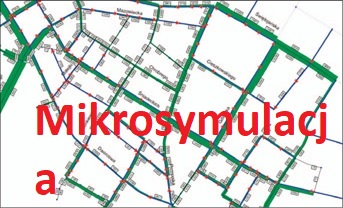
\includegraphics[width=0.8\textwidth]{Mikrosymulacja.jpg}
		\caption{\textit{Wynik mikrosymulacji ruchu drogowego wybranych skrzyżowań w Krakowie}}
		\label{fig:Mikrosymulacja}
	\end{figure}



	\section{Model ruchu bazujące na automatach komórkowych}

	Pomysł wykorzystania automatów komórkowych w symulacji ruchu drogowego spotkała się z dużym zainteresowaniem świata nauki. świadczą o tym powstałe modele, których liczba jest całkiem spora. W tabeli poniżej przedstawione zostaną wybrane modele, zaczynając od prostego modelu reprezentowanego przez ciąg komórek w jednowymiarowej tablicy, a przechodząc do najnowszych modeli, gdzie symulacja może odbywać się na drogach dwukierunkowych, skrzyżowaniach, z udziałem sygnalizacji świetlnej. \\

	\begin{table}[h]
		\centering
		\begin{tabular}{c|l}
			\textbf{Model} & \textbf{Opis modelu} \\
			Model podstawowy – model ChopardaLuthego-Queloza & Elementarny automat komórkowy zdefiniowany przez Wolframa. Przestawia ruch pojazdów na drodze jednokierunkowej i jednopasmowej. Droga wyrażona jest za pomocą jednowymiarowej tablicy, w której każda z komórek może być zajęta przez pojazd lub wolna. Odpowaida to dwóm stanom: 1 lub 0. Wszystkie samochody poruszają się w jedna stronę (np. w prawo) maksymalnie o jedną pozycję pod warunkiem, że komórka docelowa jest wolna\\
		\end{tabular}
		\caption{Modele ruchu miejskiego bazujące na automatach komórkowych}
		\label{tab:my_label}
	\end{table}





	https://www.czasopismologistyka.pl/artykuly-naukowe/send/239-artykuly-na-plycie-cd/2670-artykul









	\section{Model Nagela-Schreckenberga}

	Model ten opisuje uproszczony model poruszania się samochodów. Jednopasmowa i jednokierunkowa droga zostaje podzielona na odcinki o długości przeciętnego samochodu w raz z wolnym miejscem z przodu i z tyłu. W każdej komórce w danym czasie może znajdować się tylko jeden samochód.

	Funkcja przejścia podzielona została na etapy:

	\begin{itemize}
		\item{\textbf{Przyspieszanie} - wszystkie samochody zwiększają swoją prędkość, jeżeli do tej pory jechały z prędkością mniejszą niż maksymalna na danej ulicy.}

		\begin{equation}
			v(t+1) \rightarrow min(v(t)+1,v_{max})
		\end{equation}
		gdzie: v(t) - prędkość aktualna

		\item{\textbf{Hamowanie} - jeśli liczba komórek wolnych od samochodu do samochodu jadącego przed rozpatrywanym jest mniejsza niż prędkość samochodu, to kierowca samochodu musi dostosować prędkość, aby uniknąć kolizji.}

		\begin{equation}
			v(t+1) \rightarrow min(v(t)+1,g(t)-1)
		\end{equation}
		gdzie: g(t) - liczba pustych komórek między pojazdami

		\item{\textbf{Zdarzenia losowe} - samochód zmniejsza prędkość z uwagi na nieprzewidziane zachowanie na drodze, z określonym prawdopodobieństwem.}

		Prawdopodobieństwo $p$, że zajdzie $v(t+1) \rightarrow max(v(t)-1)>=1$.

		\item{\textbf{Przesunięcie} - wszystkie samochody przesuwają się o określony dystans, zgodnie z prędkością obliczoną w poprzednich krokach (ruch, zmiana położenia w czasie).}

		\begin{equation}
			x(t+1)=x(t)+v(t)
		\end{equation}

	\end{itemize}

	Te cztery czynności powtarza się wiele razy, tak długo, jak jest to wymagane do badania wszelkich korków, które mogą tworzyć. Model jest przykładem automatu komórkowego. Model dotyczy pojedynczego pasa, w którym samochody nie mogą się wyprzedzać.

	\begin{figure}[H]
		\centering
		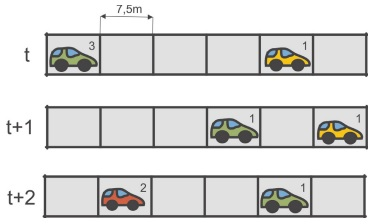
\includegraphics[width=0.8\textwidth]{N-Sch_1.jpg}
		\caption{\textit{Ruch w modelu Nagela-Schreckenberga na pasie ruchu w kolejnych chwilach czasowych}}
		[źródło: http://journals.bg.agh.edu.pl/AUTOMATYKA/2009-03/Auto43.pdf]
		\label{fig:N-Sch_1}
	\end{figure}



	\section{Planowanie i optymalizacja tras}

	Istnieje wiele sposobów na planowanie transportu min. rzędy, kolumny, tabele, wykresy. Skuteczność tych sposobów można ocenić w sposób analityczny i bez zamawiania kosztownych symulacji. Jednak przy coraz większym stopniu złożoności ruchu wyniki planowania oparte wyłącznie na skumulowanych wartościach są trudne do sprawdzenia, a co więcej są one trudne do zrozumienia. W takim przypadku rozwiązaniem pozwalającym na wyciągnięcie miarodajnych wniosków potrzebnych do podjęcia decyzji, jest graficzne przedstawienie organizacji ruchu drogowego. Mikrosymulacje:

	\begin{itemize}
		\item pozwalają na graficzne przedstawianie abstrakcyjnych danych, co ułatwia ich zrozumienie;
		\item pomagają odwzorowywać procesy organizacji ruchu;
		\item pomagają rozpoznawać potencjalnie słabe strony sieci (wraz z przyczynami);
		\item pozwalają weryfikować podjęte działania pod kątem ich wpływu na ruch drogowy.
	\end{itemize}

	Przy użyciu narzędzia do mikrosymulacji ruchu drogowego można tworzyć realistyczne wizualizacje, które ułatwią zrozumienie zachowań drogowych osobom bez technicznego przygotowania, zwłaszcza gdy w podejmowaniu decyzji udział biorą organy polityczne lub opinia publiczna. Przyszłe i jeszcze nie istniejące alternatywy staną się widoczne, a kompleksowe połączenia okażą się intuicyjne i zrozumiałe.
	Największą zaletą mikrosymulacji jest dostępność szczegółów, które można wykorzystać do budowy wirtualnej rzeczywistości. Można tworzyć symulację interakcji kierowców i pieszych w całej sieci transportowej zgodnie ze stereotypowymi zasadami przemieszczania się. Dodatkowo wizualizacja wszystkich sygnalizatorów świetlnych pozwala zobaczyć, które światła świecą na zielono, a które na czerwono. Symulacja umożliwia wprowadzenie szczegółów na poziomie zbliżonym do rzeczywistego, tak aby utworzony model miał jak najlepszą rozdzielczość.



	\section{Sygnalizacja świetlna}

	Dodatkiem do modelu Nagela-Schreckenberga może być model sygnalizacji świetlnej. Sygnalizacja jest systemem komunikującym kierowcom, możliwość kontynuowania jazdy, co wpływa na zwiększenie poziomu bezpieczeństwa.

	Aby zamodelować sygnalizację świetlną dodajemy kilka rozszeżeń do naszego modelu:
	\begin{itemize}
		\item samochód dojeżdzający do sygnalizacji świetlnej zmniejsza swoją prędkość,
		\item jeśli kierowca dojedzie do sygnalizacji, a sygnalizacja wskazuje na światło zielone, kierowca kontynuuje jazdę,
		\item jeśli kierowca dojedzie do sygnalizacji, lecz sygnalizacja wskazuje na światło czerowne, kierowca zatrzymuje się i oczekuje na światło zielone,
	\end{itemize}



	\section{Skrzyżowanie}

	\begin{itemize}
		\item Drogi dwupasmowe i dwukierunkowe przecinają się pod kątem prostym.
		\item Kolor świateł zmienia się na i-tym skrzyżowaniu co $t_{i}$ iteracji (jest to bliskie rzeczywistości rozwiązanie, ponieważ rzadko się zdarza aby sygnalizacja świetlna na dwóch różnych skrzyżowaniach, które sąsiadują ze sobą była zsynchronizowana).
		\item Odległości między poszczególnymi skrzyżowaniami mogą być różne.
		\item Komórka może być zajęta przez samochód, bądź wolna (zajęta komórka posiada wartość liczbową określającą prędkość pojazdu znajdującego się na dowolnym odcinku drogi, w danej chwili).
		\item Funkcja przejścia składa się z 4 etapów: przyśpieszenie, hamowanie, zdarzenie losowe i przesunięcie.
	\end{itemize}

	Obserwacje wynikające z symulacji skrzyżowania pokazują, że przepustowość sygnalizacji świetlnej zależy głównie od maksymalnego przyspieszenia. Dla przepustowości mniejszej od liczby samochodów chcących przejechać przez skrzyżowanie kolejka pojazdów oczekujących na przejazd będzie ulegać stopniowemu wydłużeniu. Zator powstający w ten sposób może sięgać nawet poprzedniego skrzyżowania. Model uwzględnia także występujące w rzeczywistości zachowania, tzn. postawy kierowców, którzy wjeżdżają na skrzyżowanie mimo braku możliwości jego opuszczenia. Konsekwencją takiego zachowania jest blokada przejazdu dla innych użytkowników ruchu, co prowadzi do zmniejszenie przepustowości sygnalizacji świetlnej. Ponad to powstający w ten sposób zator posiad tendencje do rozprzestrzeniania się ze względu na to, że jest to system naczyń połączonych. W wyniku takiego zachowania jednostkowa sytuacja może prowadzić do paraliżu całego układu komunikacyjnego badanego obszaru. \\*

	\textbf {Reguły ruchu na skrzyżowaniu} \\*

	Możliwość dostosowania modelu do potrzeb konkretnego rozwiązania wymaga użycia wielu parametrów konfiguracyjnych dla pasów ruchu i poszczególnych typów pojazdów. Organizacja ruchu na skrzyżowaniu wymaga zastosowania dodatkowych reguł ruchu pojazdów, uwzględniających zasady ruchu na nim. Bezpieczna prędkość wymaga zastosowania procedur umożliwiających jej określenie dla każdej sytuacji ruchowej.

	\begin{itemize}
		\item{\textbf{Prędkość ruchu pojazdów}}
	\end{itemize}

	Pojazdy mogą się poruszać z prędkością od 0 do 5 m/s. Mniejsze prędkości od dopuszczalnych prędkości ruchu dla poszczególnych typów pojazdów można uzyskać dzięki wprowadzeniu zdarzenia losowego tj. np.: prawdopodobieństwa zahamowania wynikającego z panujących warunków pogodowych.

	\begin{itemize}
		\item{\textbf{Bezpieczna prędkość ruchu pojazdów}}
	\end{itemize}

	Każdy pojazd potrafi określić swoją bezpieczną prędkość, czyli zachować bezpieczny odstęp od poprzedniego pojazdu, zmniejszyć prędkość albo zatrzymać się w określonej komórce drogi. Funkcja określająca drogę hamowania zależy od bieżącej prędkości pojazdu i w przypadku wykorzystania idealnego opóźnienia hamowania dla b=1 m/s może mieć postać:

	\begin{equation}
		S_{b}(v)=\sum_{i=1}^{v-1} i[komórek]
	\end{equation}

	Chcąc uwzględnić stan nawierzchni czy też warunki pogodowe uniemożliwiające idealne hamowanie funkcję (1) należy uzupełnić o współczynniki korygujące drogę hamowania.
	W przeciętnych warunkach ruchu czas reakcji kierowcy przyjmowany jest jako 1 s, ale możliwe jest jego zwiększenie w niekorzystnych warunkach ruchu.
	Każdy pojazd potrafi utrzymywać bezpieczną odległość, zmniejszając ją w przypadku obecności pojazdu poprzedzającego, utrzymując ją oraz próbując przyspieszyć, gdy jego prędkość jest mniejsza od lokalnie dopuszczalnej.

	\begin{itemize}
		\item{\textbf{Przejazd przez skrzyżowanie}}
	\end{itemize}

	Prędkości przejazdu pojazdów przez skrzyżowanie z prędkością większą od 1 m/s [\textit{Rys. 1}] dopuszcza są w przypadku przejazdu przez skrzyżowanie na wprost drogą nadrzędną oraz podczas sygnału zielonego.

	\begin{figure}[H]
		\centering
		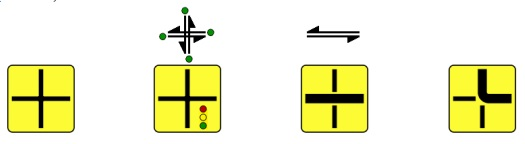
\includegraphics[width=0.8\textwidth]{S1.jpg}
		\caption{\textit{Przypadki przejazdu pojazdów przez skrzyżowanie z prędkością większą niż 1 m/s}}
		[\small{źródło: https://www.czasopismologistyka.pl/artykuly-naukowe/send/318-artykuly-na-plycie-cd-3/7028-artykul}]
		\label{fig:S1}
	\end{figure}

	[\textit{Rys. 2}] przedstawia tory ruchu po skrzyżowaniu dla pojazdów różnych relacji. Rozpatrując przypadek załamanego przebiegu drogi z pierwszeństwem przejazdu, skręt w lewo zostaje zrealizowany bez przekroczenia osi jezdni nadrzędnej.

	\begin{figure}[H]
		\centering
		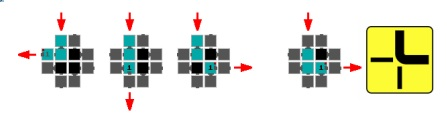
\includegraphics[width=0.8\textwidth]{S2.jpg}
		\caption{\textit{Tory przejazdu przez skrzyżowanie}}
		[\small{źródło: https://www.czasopismologistyka.pl/artykuly-naukowe/send/318-artykuly-na-plycie-cd-3/7028-artykul}]
		\label{fig:S2}
	\end{figure}

	W celu urzeczywistnienia przejazdu przez tak małe skrzyżowanie pojazdów ciężkich, dodatkowo należy sprawdzić czy wszystkie części ciężkiego pojazdu opuściły obszar skrzyżowania właściwego, ponieważ dopiero wtedy zwiększenie prędkości takiego pojazdu do wartości większych niż 1 m/s jest możliwe. Działanie takiego algorytmu przedstawia [\textit{Rys. 3}].

	\begin{figure}[H]
		\centering
		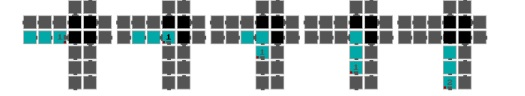
\includegraphics[width=0.8\textwidth]{S3.jpg}
		\caption{\textit{Przejazd pojazdu ciężkiego przez skrzyżowanie}}
		[\small{źródło: https://www.czasopismologistyka.pl/artykuly-naukowe/send/318-artykuly-na-plycie-cd-3/7028-artykul}]
		\label{fig:S3}
	\end{figure}


	\begin{itemize}
		\item{\textbf{Wjazd na skrzyżowanie}}
	\end{itemize}

	Zbliżający się do skrzyżowania pojazd musi ustąpić pierwszeństwa przejazdu zgodnie z zasadami wynikającymi z rodzaju skrzyżowania i organizacji ruchu na nim. W przypadku organizacji ruchu i relacji zbliżając się końca wlotu pojazd kontroluje swoją prędkość tak, aby w ostatniej komórce wlotu przed skrzyżowaniem wynosiła 1 m/s. Dzięki temu możliwe jest ewentualne zatrzymanie pojazdu przed skrzyżowaniem i ustąpienie pierwszeństwa przejazdu. Bezwzględne zatrzymanie pojazdu występuje jeżeli wlot jest podporządkowany znakiem „stop” lub jeżeli wyświetlany jest inny sygnał niż zielony (pojazd, który nie jest w stanie się zatrzymać przed skrzyżowaniem przejeżdża przez nie). Pojazd zmuszony do zatrzymania musi odczekać założoną ilość czasu zanim włączy się do ruchu.

	Zbliżając się do skrzyżowania pojazd musi podjąć odpowiednie decyzje. Schemat postępowania zależy wtedy od organizacji ruchu, jednak główne kroki w takim przypadku są następujące:

	\begin{enumerate}
		\item sprawdzenie obecności pojazdów, które nie opuściły skrzyżowania,
		\item sprawdzenie możliwości przejazdu przez skrzyżowanie i jego opuszczenia,
		\item sprawdzenie pierwszeństwa przejazdu.
	\end{enumerate}

	\begin{itemize}
		\item{\textbf{Wpływ pieszych na ruch pojazdów}}
	\end{itemize}

	W modelu zakłada się respektowanie pierwszeństwa pieszych na przejściach zlokalizowanych na wlotach, wylotach i dodatkowych pasach ruchu. Każde wyznaczone przejście posiada dwa parametry: czas zablokowania przejścia, a także prawdopodobieństwo pojawienia się pieszego, czy też grupy pieszych.

	\section{Symulacja zjawiska}

	\textbf{\normalsize{Wybór języka programowania}}

	Symulator ma za zadanie na wielu płaszczyznach wspierać możliwości rozszerzania. Obecnie za paradygmat programowania pozwalający na rozszerzenie funkcjonalności w uważa się paradygmat programowania obiektowego, dlatego pod uwagę przy wyborze języka programowania brane były języki związane z tym paradygmatem oraz znane przynajmniej w podstawowym stopniu członkom projektu. Pod uwagę wzięto: C++, Java, C\#.

	Istotnym elementem z punktu widzenia każdej aplikacji jest możliwość jej wykorzystania na różnych platformach sprzętowo-systemowych. C++ i Java zdają się pokrywać zakresem dostępności (porównywalna ilości platform). Natomiast C\# wydaje wydaje się nie być dostępny na wielu platformach tj. Java i C++. Z tego powodu C\# został odrzucony i nie będzie rozpatrywany w kolejnych kategoriach doboru.

	Kolejnym aspektem jest wydajność obliczeń. Nie jest ona kluczowym elementem dla aplikacji, ale czas obliczeń to kosz, dlatego minimalizacja czasu wydaje być istotnym elementem przy doborze języka programowania. W tej kategorii przewaga C++ nad Javą jest niezaprzeczalna. Z drugiej strony wydajność to nie główne kryterium doboru technologii, dlatego nie zdecydowano się na odrzucenie tego języka na tym etapie.

	Błędy programistyczne to nieodłączny element pisania aplikacji. Języki różnego typu bronią się przed tymi błędami na różne sposoby. Za błąd w tych językach uważa się zachowania powszechnie uznawane za nielogiczne, np.: stawianie obiektów złych klas w nieokreślonych dla nich kontekstach. C++ posiada ręczne zarządzanie pamięcią, które jest uznawane za jeden z najbardziej błędogennych elementów tworzenia oprogramowania, dlatego w tej kategorii Java (sam obsługujący zarządzanie pamięcią nie obciążając tym zadaniem programisty) wydaje się być lepszy.

	Biorąc pod uwagę powyższe kryteria oceny wybrano język \textbf{Java}. Kluczowe okazało się doświadczenie programistyczne autorów pracy. Wydajność obliczeniowa w dzisiejszych czasach nie jest wysokim kosztem, a dla naszego projektu nie jest kluczowa. Dodatkowo język chroniący programistę przed własnymi błędami ma wg autorów sporą przewagę. \\*

	\textbf{\normalsize{Diagramy statyczne UML}}

	tu bd opis pakietów, klas, implementacji




	\section{Wyniki symulacji}

	Opracowan w pracy model skrzyżowania obrazuje sumulację ruchu ulicznego samochodów w mieście - MIKROSYMULACJA. Uzyskane w pracy wyniki obrazuje animacja pokazująca jak wygląda ruch na skrzyżowaniu (Załącznik 3).

	Dzięki symulacji możliwe jest uwidocznienie zjawiska blokowania się skrzyżowań. To zjawisko zostało rozwiązane poprzez zaprogramowanie sygnalizacji świetlnej, która w przypadku jak na rysunku poniżej, wymusza zatrzymanie pojazdu na czerwonym świetle.

	\begin{figure}[H]
		\centering
		
\includegraphics[width=0.8\textwidth]{Wyniki_sym_1.jpg}
		\caption{\textit{Widok skrzyżowania z sygnalizacją świetlną}}
		\label{fig:Wyniki_sym_1}
	\end{figure}



	\section{Podsumowanie}

	Uruchamiając symulację zaimplementowaną w sposób przedstawiony powyżej zauważamy, że nawet tak prosty model ruchu samochodów jest w stanie, z pewnym przybliżeniem, odwzorować zachowanie kierowców podczas przejazdu przez skrzyżowanie. Symulacja pozwala również dostosowywać działanie świateł na podstawie obserwowania zagęszczenia ruchu na poszczególnych ulicach i badać skutki, do jakich te zmiany doprowadzają. Mimo, że na drodze nie dochodzi do łamania przepisów przez kierowców wszystkie pojazdy są reprezentowane poprzez punkty, nie uwzględniając ich długości, nie uwzględnione zostały również umiejętności i poziom odwagi kierowców. Jednak wszystkie te czynniki mogą zostać w przyszłości zaimplementowane i dzięki temu model może okazać się jeszcze bardziej odpowiadający rzeczywistemu zachowaniu na drodze.

	Istnieje wiele możliwości rozbudowania opracowywanego środowiska do symulacji ruchu drogowego.W przyszłości może ono posiadać m.in możliwości wykorzystania:
	\begin{itemize}
		\item dodanie innych użytkowników ruchu tj.: pieszych, rowerzystów, ciężkich aut, a także komunikacji zbiorowej (tramwaje, autobusy);
		\item dostępu z poziomu przeglądarki www;
		\item rozbudowanego  edytora map, dzięki któremu można modelować;
		\item dowolnego obszaru objętego badaniem np. konfliktowych skrzyżowań dróg;
		\item procesu symulacji, który umożliwia np. zróżnicowanie samochodów ze względu na różne wartości maksymalnych przyspieszeń czy prędkości, generowanie zdarzeń losowych, czy modelowanie specyficznych sytuacji na drodze;
		\item statystyki oraz wizualizacja danych wygenerowanych przez symulator min. tj.: natężenie ruchu, średnia prędkość, wartości prędkości i przyspieszeń pojazdów na danym odcinku drogi, czy też przepustowość danego obszaru;.
	\end{itemize}

	\newpage
	\section{Załączniki}

	\begin{itemize}
		\item Załącznik 1 \textit{Wersja wykonywalna}
		\item Załącznik 2 \textit{Kody źródłowe wraz z komentarzami}
		\item Załącznik 3 \textit{Animacja ruchu ulicznego na skrzyżowaniu z sygnalizacją świetlną}
	\end{itemize}


	\newpage
	\section{Bibliografia}

	\begin{itemize}
		\item Bartodzieja Maciej: \textit{Modelowanie ruchu ulicznego za pomocą automatów Komórkowych}, Wrocław 2007, Praca Dyplomowa napisana pod kierunkiem: dr Rafała Werona;
		\item Smoczyński Mariusz \textit{Automat komórkowy w modelowaniu ruchu na małym skrzyżowaniu};
		\item Małecki Krzysztof, Rokita Mateusz, Wątróbski Jarosław: \textit{Wykorzystanie automatów komórkowych w modelowaniu ruchu drogowego}, wyd. ZUT, Szczecin;
		\item Andrzej Fiedukowicz: \textit{Implementacja symulatora ruchu obiektów w środowisku miejskim na potrzeby systemu fuzji danych}, praca inżynierska pod opieką dr inż. Rafała Biedrzyckiego, PW WEiTI, 2013 r.;
		\item Stanisław Krawiec, Ireneusz Celiński: \textit{Symulacja mikroskowpowa ruchu w modelu obszarowym sieci drogowej}, praca naukowa Politechniki Warszawskiej, 2012 r.;
		\item http://journals.bg.agh.edu.pl/AUTOMATYKA/2009-03/Auto43.pdf, data dostępu: 05.01.2019 r.;
		\item https://www.czasopismologistyka.pl/artykuly-naukowe/send/338-artykuly-na-plycie-cd-2/9439-maciejewski-maciejewski-zintegrowana-symulacja-i [data dostępu: 09.01.2019 r.];
		\item Maciejewski M.: \textit{Zastosowanie automatów komórkowych do symulacji ruchu drogowego w mieście}, 'Logietyka', 2010, nr 2
		\item Maciejewski Marek, Maciejewski Tomasz: \textit{Uwarunkowanie makroskopowych modei ruchu drogowego}, Prace naukowe Politechniki Warszawskiej, 2013, str. 309-310 [źródło: \textit{http://docplayer.pl/59926749-Uwarunkowanie-makroskopowych-modeli-ruchu-drogowego.html}];
		\item Małecki Krzysztof, Szmajdziński Maciej: \textit{Symulator do mikroskopowej analizy ruchu drogowego}, str. 1435-1438 [źródło: \textit{https://www.czasopismologistyka.pl/artykuly-naukowe/send/239-artykuly-na-plycie-cd/2670-artykul}];
	\end{itemize}

\end{document}
